\documentclass[11pt]{article}
\usepackage[margin=2.2cm]{geometry}
\usepackage{graphicx,booktabs,amsmath,amssymb,amsthm,enumitem,float,xcolor,caption,microtype,array}
\usepackage{url}
\usepackage[hidelinks]{hyperref}
\usepackage{tikz}
\usetikzlibrary{arrows.meta,positioning,shapes.geometric}
\captionsetup{font=small,labelfont=bf}
\setlist{itemsep=2pt,topsep=4pt}
\newcommand{\kA}{k_A}
\newcommand{\kG}{k_G}
\newcommand{\xc}{x_{0,\mathrm{crit}}}
\newcommand{\zsn}{z_{\mathrm{SN}}}
\newcommand{\xsn}{x_{1,\mathrm{SN}}}
\newcommand{\xh}{x_0^{\mathrm{HSP}}}
\newtheorem*{remark}{Remark}
\definecolor{boxc}{HTML}{F4F3EF}
\newcommand{\keybox}[1]{\par\noindent\colorbox{boxc}{\parbox{\dimexpr\linewidth-2\fboxsep}{\small #1}}\par\medskip}

\title{The Epileptor, and what it means to place a homeostatic-plasticity\\ seizure cycle in its coordinates}
\author{}
\date{Working notes accompanying \texttt{HSP\_Epileptor\_trajectory.ipynb}}

\begin{document}
\maketitle
\tableofcontents
\newpage

%==========================================================================================
\section{Why connect the two models}
%==========================================================================================
Our spiking E/I network with homeostatic synaptic plasticity (HSP) produces seizures \emph{mechanistically}: under
a reduced drive (36\,Hz instead of 40\,Hz), HSP slowly raises recurrent excitation ($\kA\uparrow$) and lowers
inhibition ($\kG\downarrow$) until the network ignites into a high-rate state; the over-activity then makes HSP
collapse excitation, which ends the seizure and leaves a long post-ictal depression. The cycle repeats every
1--2 hours (HSP time constants of 250\,s).

The \emph{Epileptor} \cite{jirsa2014} is the opposite kind of model: phenomenological, a handful of
differential equations built to reproduce the \emph{dynamical signature} of seizures (how they start, how they
end, how they recur), without committing to a biophysical mechanism. Its parameters have become a common language
in computational epileptology: the excitability $x_0$ is what the Virtual Epileptic Patient pipeline infers for each
brain region to delineate the epileptogenic zone \cite{jirsa2017,proix2017}.

Placing the HSP cycle in Epileptor coordinates asks a precise question:
\keybox{\textbf{Does HSP act as a mechanistic slow variable that moves the network through the Epileptor's
seizure-generating bifurcation, and if so, does it play the role of the excitability $x_0$, of the permittivity
variable $z$, or of both?}}
The mapping is \emph{post hoc}: nothing is fed back into the spiking network. We only re-express its recorded
trajectory in Epileptor variables and check whether the Epileptor geometry (fold, critical $x_0$, slow
nullcline) organises it.

%==========================================================================================
\section{The Epileptor}
%==========================================================================================
\subsection{Where it comes from: a bifurcation taxonomy of seizures}
Jirsa et al. \cite{jirsa2014} started from a dynamical-systems observation. A seizure is a transition between
two states of a neural population, a resting (interictal) state and an oscillatory (ictal) state, and such
transitions are \emph{bifurcations} of a fast subsystem driven by a slower variable. The kind of bifurcation leaves
fingerprints in the recordings:
\begin{itemize}
\item \textbf{Onset by a saddle-node bifurcation}: a rest state and a saddle collide and disappear; the system jumps to
an oscillation whose amplitude is finite immediately and whose baseline shifts. This matches the \emph{DC shift}
often seen at seizure onset.
\item \textbf{Offset by a homoclinic bifurcation}: the oscillation ends when the limit cycle collides with a saddle;
the inter-spike interval grows logarithmically as the bifurcation is approached, i.e. the discharge
\emph{slows down} before stopping, while the amplitude stays roughly constant. This matches the
frequency-slowing at the end of many focal seizures.
\end{itemize}
A fast subsystem that is pushed back and forth through a saddle-node (onset) and a homoclinic (offset) bifurcation
by a slow variable is a \emph{square-wave burster} in Izhikevich's classification of bursters \cite{izhikevich2000}.
The Epileptor is the minimal model of that class with the additional ingredients needed to reproduce human and animal
seizure recordings. Later work generalised the idea to a full taxonomy of 16 onset/offset ``dynamotypes'', among which
the Epileptor's saddle-node/homoclinic pair is one of the most frequently observed in patient recordings \cite{saggio2020}.

\subsection{The full model (five state variables plus a filter)}
With TVB's default parameters \cite{sanzleon2013}:
\begin{align}
\dot x_1 &= y_1 - f_1(x_1, x_2, z) - z + I_{ext,1}, &
\dot y_1 &= c - d\,x_1^2 - y_1, \label{eq:pop1}\\
\dot z   &= r\,\big[\,s\,(x_1 - x_0) - z - 0.1\,z^7\,\mathbf 1_{z<0}\big], \label{eq:z}\\
\dot x_2 &= -y_2 + x_2 - x_2^3 + I_{ext,2} + b_2\, g - 0.3\,(z - 3.5), &
\dot y_2 &= \tfrac{1}{\tau_2}\,\big(-y_2 + f_2(x_2)\big), \label{eq:pop2}\\
\dot g &= -0.01\,(g - 0.1\,x_1), \label{eq:g}
\end{align}
with
\[
f_1 = \begin{cases} a x_1^3 - b x_1^2, & x_1 < 0\\ -\big(\mathrm{slope} - x_2 + 0.6\,(z-4)^2\big)\,x_1, & x_1\ge 0\end{cases}
\qquad
f_2 = \begin{cases} 0, & x_2 < -0.25\\ a_2\,(x_2 + 0.25), & x_2 \ge -0.25.\end{cases}
\]
Parameters: $a=1$, $b=3$, $c=1$, $d=5$, $s=4$, $I_{ext,1}=3.1$, $I_{ext,2}=0.45$, $\tau_2=10$, $a_2=6$,
$b_2=2$, slope $=0$, $r=0.00035$, and $x_0$ (TVB default $-1.6$; the critical value is near $-2.06$, see below).

\begin{table}[H]\centering\small
\begin{tabular}{>{\raggedright}p{2.7cm}>{\raggedright}p{3.3cm}p{8.6cm}}
\toprule
variables & name & role \\
\midrule
$(x_1, y_1)$ & population 1 & fast discharges; its bistability (rest vs oscillation) creates onset and offset \\
$(x_2, y_2)$ & population 2 & slower spike-and-wave events ($\tau_2=10$) superimposed during the seizure \\
$g$ & low-pass coupling & population 1 drives population 2 through a slow filter of $x_1$ \\
$z$ & \emph{permittivity} (slow) & time scale $1/r \approx 2857$ units; integrates $x_1$ and moves population 1 across its bifurcations \\
$x_0$ & excitability (parameter) & position of the slow nullcline; decides whether a stable rest state exists \\
\bottomrule
\end{tabular}
\caption{The Epileptor's subsystems.}
\end{table}

\textbf{How a seizure unfolds} (Fig.~\ref{fig:6d}). Between seizures, $x_1$ sits at a rest state on the left
branch of population 1's nullcline, and $z$ slowly \emph{decreases} (because $s(x_1 - x_0) < z$ there). When $z$ falls
below the saddle-node value, the rest state disappears: $x_1$ jumps to the oscillatory branch (onset: DC shift and fast
discharges), population 2 starts producing spike-wave events, and $z$ now \emph{increases}, since $x_1$ is high. Rising
$z$ moves population 1 towards the homoclinic bifurcation, the discharges slow down and stop (offset), and $x_1$ falls
back to rest, where $z$ decreases again. The seizure is thus a hysteresis loop of the fast subsystem, driven by $z$.
$z$ is a \emph{negative feedback} that accumulates during the seizure and terminates it; it has been interpreted as a
slow process such as changes in extracellular ion concentrations or energy metabolism, but the model does not depend
on that interpretation \cite{jirsa2014}.

\begin{figure}[H]\centering
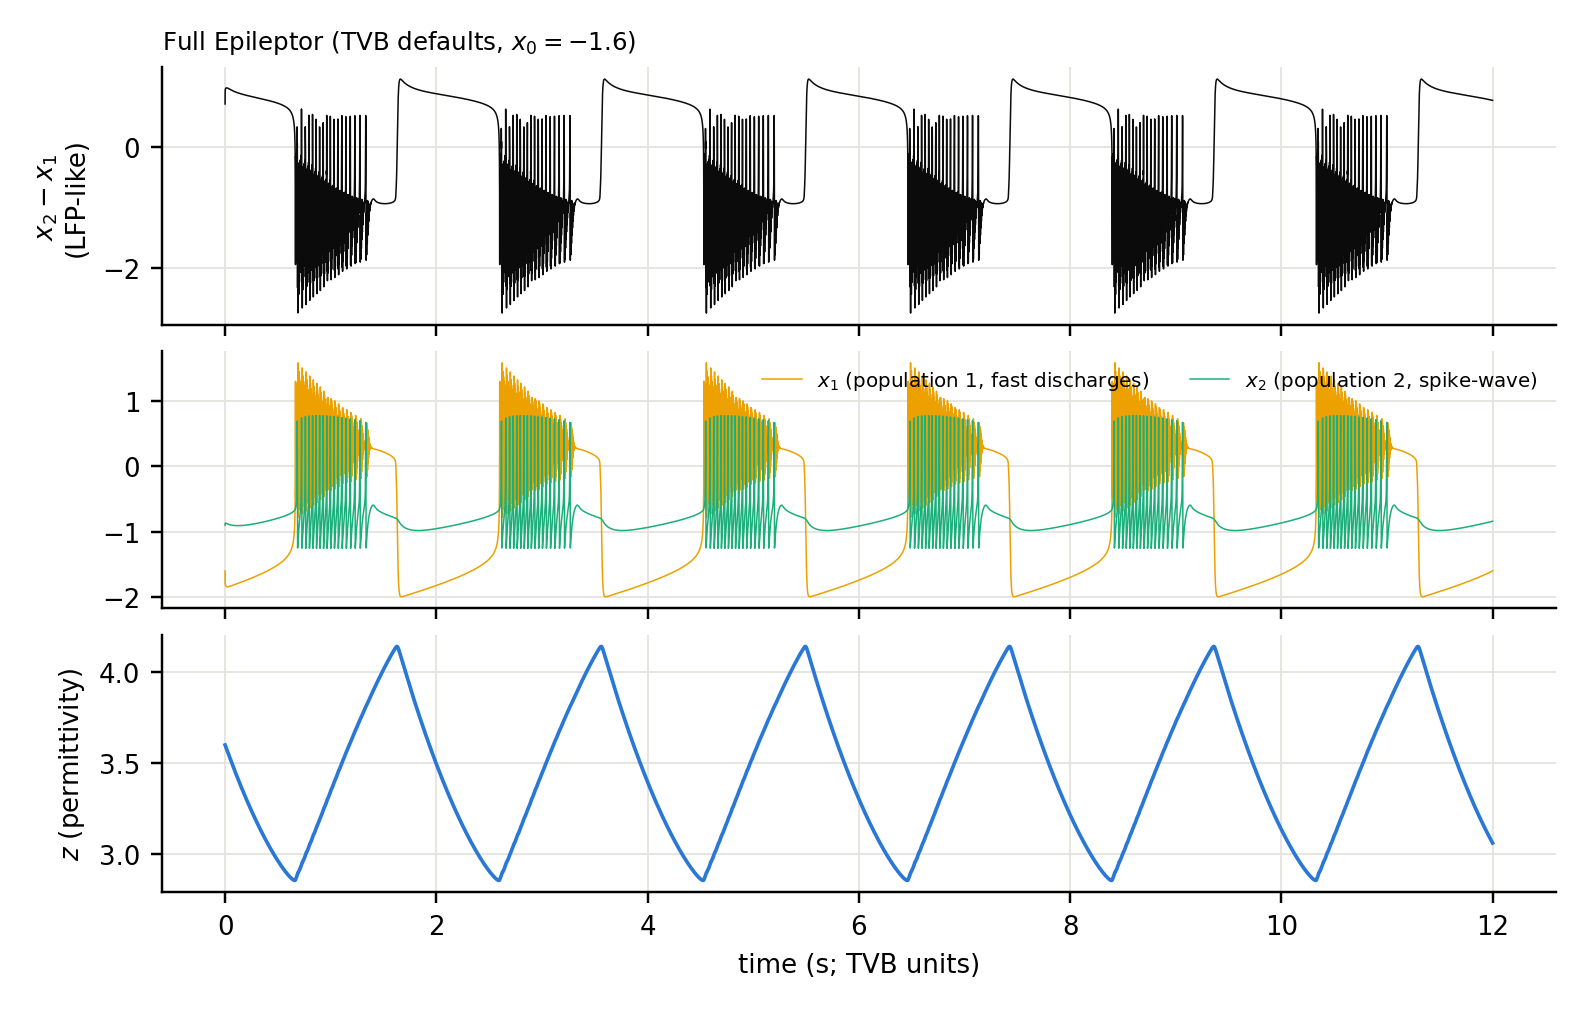
\includegraphics[width=0.95\linewidth]{figs/th_6d.png}
\caption{The full Epileptor with TVB defaults ($x_0=-1.6$, supercritical), integrated with LSODA. Top: the LFP-like
signal $x_2 - x_1$, with the DC shift at onset, fast discharges and spike-wave complexes. Middle: the two populations.
Bottom: $z$ is a sawtooth: it falls between seizures and rises during them. In TVB units (1 unit $=$ 1\,ms) a
seizure lasts $\sim0.7$\,s; in practice the time axis is rescaled to the data.}\label{fig:6d}
\end{figure}

\textbf{Time units.} The Epileptor equations have no intrinsic time unit. TVB integrates them with the step in
milliseconds and $r=0.00035$, i.e.\ $1/r\approx2.9$\,s. Seizure duration and recurrence scale with $1/r$ and with
$x_0$, so when fitting data the time axis (or $r$) is usually rescaled. This matters for us (Section~\ref{sec:timescales}).

\subsection{The excitability $x_0$ and the slow nullcline}
$x_0$ appears only in the $z$ equation \eqref{eq:z}. Setting $\dot z=0$ gives the \emph{slow nullcline}
$z = s(x_1 - x_0)$, a straight line of slope $s=4$; increasing $x_0$ shifts it to the right (or down). The rest state
is the intersection of this line with the left (interictal) branch of the fast nullcline. If the line intersects
the branch to the left of its fold, the intersection is a stable fixed point and the region rests indefinitely
(\emph{subcritical}). If $x_0$ is large enough that the line passes the fold, there is no stable rest state on that
branch, and the region seizes periodically on its own (\emph{supercritical}). This is why, in the Virtual Epileptic
Patient, $x_0$ is the quantity that labels a region as epileptogenic (above the critical value), as part of the
propagation zone (close below it, so that input from other regions can push it over), or healthy (far below)
\cite{jirsa2017,proix2017}.

\subsection{The 2D reduction used here}
Proix et al. \cite{proix2014} reduced the Epileptor to two variables to study seizure propagation across regions.
Two steps:
\begin{enumerate}
\item $y_1$ is fast compared with $z$; on the interictal branch it relaxes to $y_1 = c - d x_1^2 = 1 - 5x_1^2$.
\item Population 2 and the filter are dropped (they shape the ictal waveform, not the onset).
\end{enumerate}
Substituting $y_1$ and the $x_1<0$ form of $f_1$ into \eqref{eq:pop1}:
\[
\dot x_1 = (1 - 5x_1^2) - (x_1^3 - 3x_1^2) - z + I_{ext}
        = -x_1^3 - 2x_1^2 + 1 - z + I_{ext},
\]
\begin{equation}\boxed{\;\dot x_1 = -x_1^3 - 2x_1^2 + 1 - z + I_{ext}, \qquad
\dot z = r\left[\,4(x_1 - x_0) - z - 0.1\,z^7\mathbf 1_{z<0}\right]\;}\label{eq:2d}\end{equation}
($I_{ext}=3.1$, $r=0.00035$; in network versions a coupling term is added to $\dot z$, the ``permittivity coupling'' by
which a seizing region recruits its neighbours \cite{proix2014}; we have a single region and no coupling).
The fast equation is now a cubic for all $x_1$. Its upper branch replaces the oscillatory branch of the full model:
the 2D reduction keeps the \emph{onset} geometry exactly, but the homoclinic offset becomes a second fold (end of the
upper branch) and the ictal fast oscillations are averaged out.

\subsection{The fold and the critical excitability}\label{sec:fold}
Write the fast nullcline ($\dot x_1=0$) as $z = G(x_1) := -x_1^3 - 2x_1^2 + 1 + I_{ext}$. Its turning points satisfy
\[
G'(x_1) = -3x_1^2 - 4x_1 = 0 \quad\Rightarrow\quad x_1 = 0 \ \ \text{or}\ \ x_1 = \xsn = -\tfrac43 .
\]
$G''(-4/3) = -6(-4/3) - 4 = 4 > 0$: $x_1=-4/3$ is a local minimum of $G$, the lower end (fold) of the interictal
branch $x_1 < -4/3$; $x_1 = 0$ is a local maximum, the upper end of the ictal branch $x_1>0$. The fold value is
\[
\zsn = G(-\tfrac43) = \tfrac{64}{27} - \tfrac{32}{9} + 1 + I_{ext} = I_{ext} - \tfrac{5}{27} = 2.91481,
\qquad G(0) = 1 + I_{ext} = 4.1 .
\]
For fixed $z$, the fast subsystem has an interictal rest state only if $z \ge \zsn$ (the lower root of $G(x_1)=z$
exists), and an ictal state only if $z \le 4.1$. The slow nullcline passes through the fold when
$\zsn = 4(\xsn - x_0)$:
\begin{equation}\boxed{\;\xc = \xsn - \frac{\zsn}{4} = -\frac43 - \frac{I_{ext} - 5/27}{4} = -2.06204\;}\label{eq:xc}\end{equation}

\textbf{Stability (a subtlety).} With slope 4, the slow nullcline crosses the cubic exactly once, for every $x_0$
(Fig.~\ref{fig:bif}): the 2D system has a \emph{single} fixed point $(x_1^*, z^*)$, which never disappears. Its
Jacobian is
\[
J = \begin{pmatrix} G'(x_1^*) & -1 \\ 4r & -r\end{pmatrix},\qquad
\det J = r\,\big(3x_1^{*2} + 4x_1^* + 4\big) > 0,\qquad \operatorname{tr} J = G'(x_1^*) - r .
\]
The determinant is always positive (the quadratic has no real root), so there is no saddle-node of the full system.
Stability is lost when the trace changes sign, $G'(x_1^*) = r$, i.e.\ when the fixed point moves past the fold onto the
middle (repelling) branch: a Hopf bifurcation at $x_1^* \approx -4/3 + r/4$, which is within $O(r)\sim10^{-4}$ of $\xc$.
Because $r$ is tiny, this Hopf is \emph{singular}: the cycle born there explodes, over an exponentially small range of
$x_0$, into the large relaxation oscillation (a canard explosion \cite{krupa2001,kuehn2015}). So the ``saddle-node''
in the Epileptor's description refers to the \emph{fast} subsystem ($x_1$ at fixed $z$), whose rest state collides
with a saddle at $z=\zsn$; the full 2D system switches from rest to seizures at $x_0 \approx \xc$ through the
fixed point crossing that fold. In the limit $r\to0$ the two pictures coincide, and $\xc$ is the onset threshold.

\begin{figure}[H]\centering
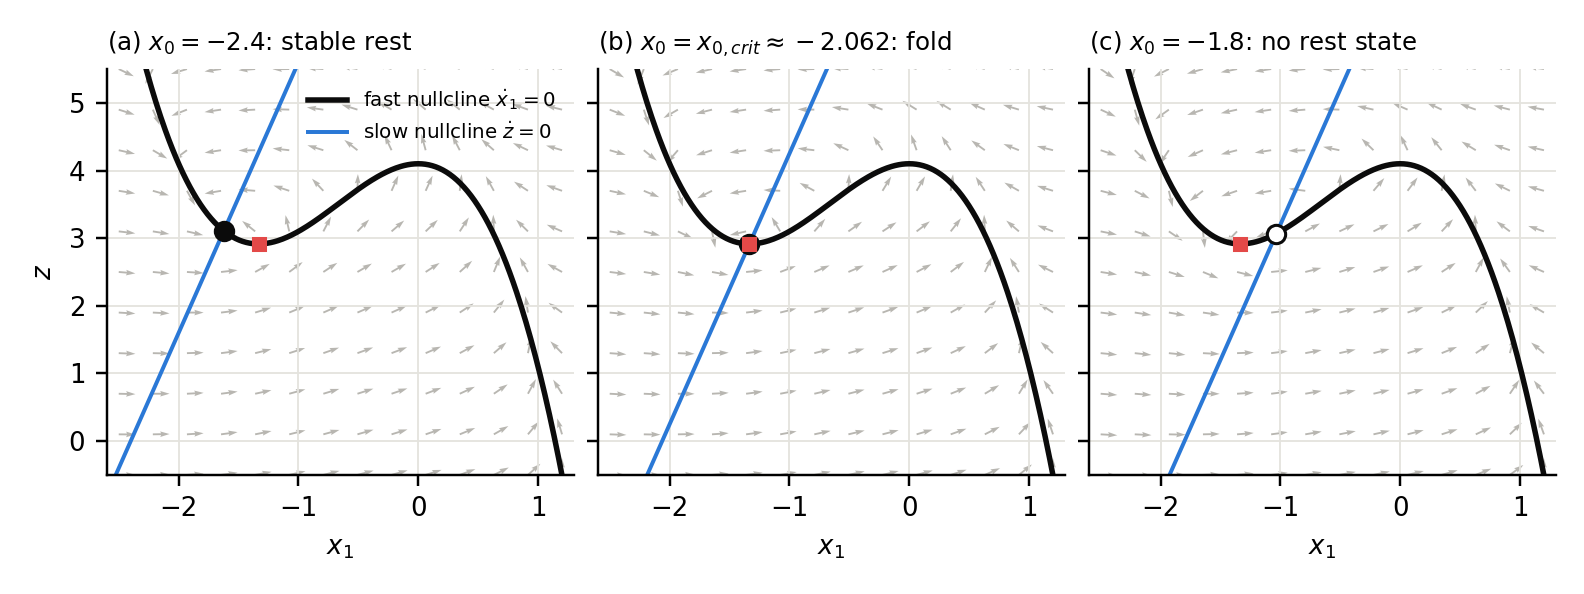
\includegraphics[width=\linewidth]{figs/th_phase_planes.png}
\caption{Phase planes of the 2D Epileptor. Black: fast nullcline $z = G(x_1)$; blue: slow nullcline
$z = 4(x_1 - x_0)$; red square: the fold $(\xsn, \zsn)$; filled/open circle: stable/unstable fixed point; grey arrows:
direction of the flow (slow component exaggerated 400$\times$). (a) Subcritical: the rest state is on the interictal
branch. (b) Critical: the slow nullcline passes through the fold. (c) Supercritical: the only fixed point is on the
repelling middle branch, so the system oscillates.}\label{fig:phase}
\end{figure}

\begin{figure}[H]\centering
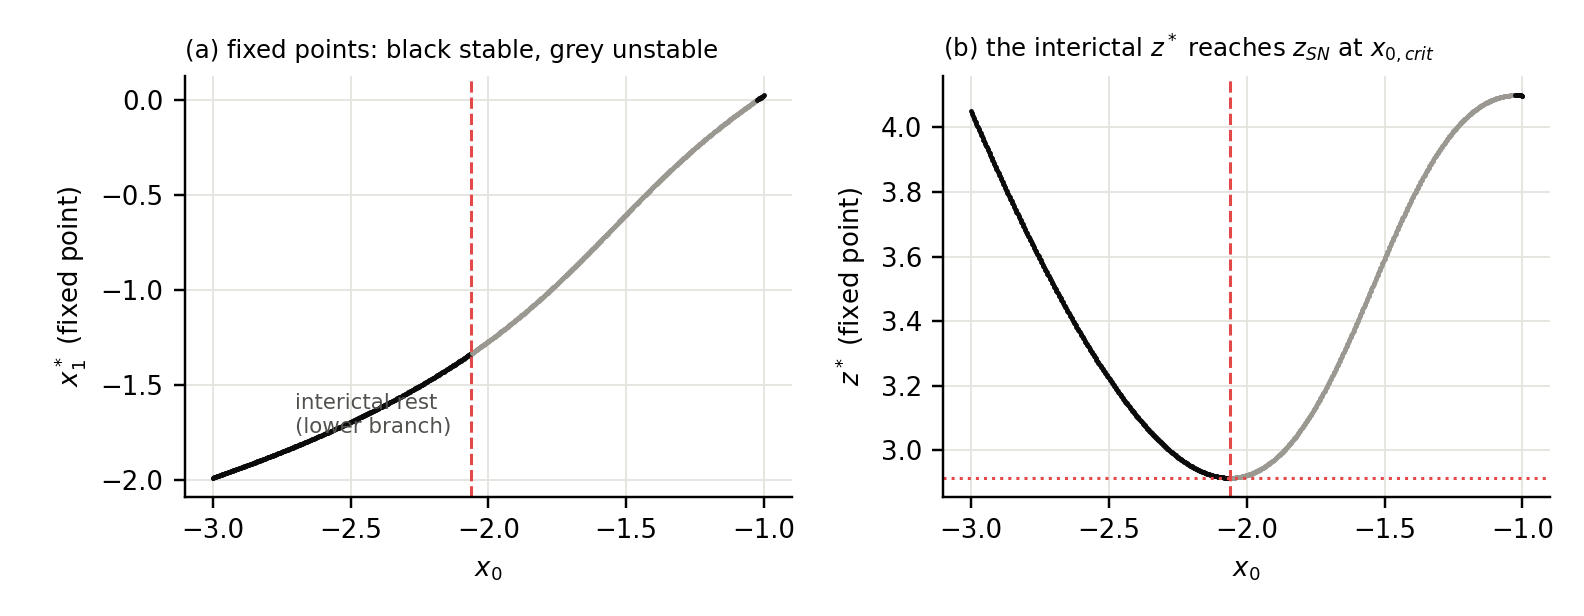
\includegraphics[width=\linewidth]{figs/th_bifurcation.png}
\caption{Fixed point of the 2D Epileptor against $x_0$. It is unique and moves continuously; it is stable (black) on
the interictal branch and loses stability at $\xc$ (red dashed). (b) At $\xc$, $z^*$ reaches its minimum $\zsn$
(dotted).}\label{fig:bif}
\end{figure}

\subsection{Relaxation oscillations: what a ``seizure'' is in the 2D model}
For $x_0 > \xc$ the trajectory follows a relaxation cycle (Fig.~\ref{fig:relax}a):
\begin{enumerate}
\item On the interictal branch, $4(x_1 - x_0) < z$, so $z$ decreases slowly while $x_1$ tracks the branch.
\item At $z=\zsn$ the branch ends: $x_1$ jumps (fast) to the ictal branch, $x_1\approx0.67$. \emph{Onset.}
\item On the ictal branch, $4(x_1 - x_0) \gg z$, so $z$ rises.
\item At $z = 4.1$ the ictal branch ends: $x_1$ jumps back to the interictal branch, $x_1 = -2$. \emph{Offset.}
\end{enumerate}
Fig.~\ref{fig:2d} shows the corresponding time series. Two properties matter for us.
\emph{Slow passage}: when $x_0$ is ramped slowly through $\xc$, onset occurs slightly after the crossing (the
trajectory stays near the vanishing rest state for a while), and seizures stop slightly after $x_0$ comes back
below $\xc$. \emph{Determinism}: without noise, the 2D Epileptor seizes as soon as, and as long as, $x_0 > \xc$.

\begin{figure}[H]\centering
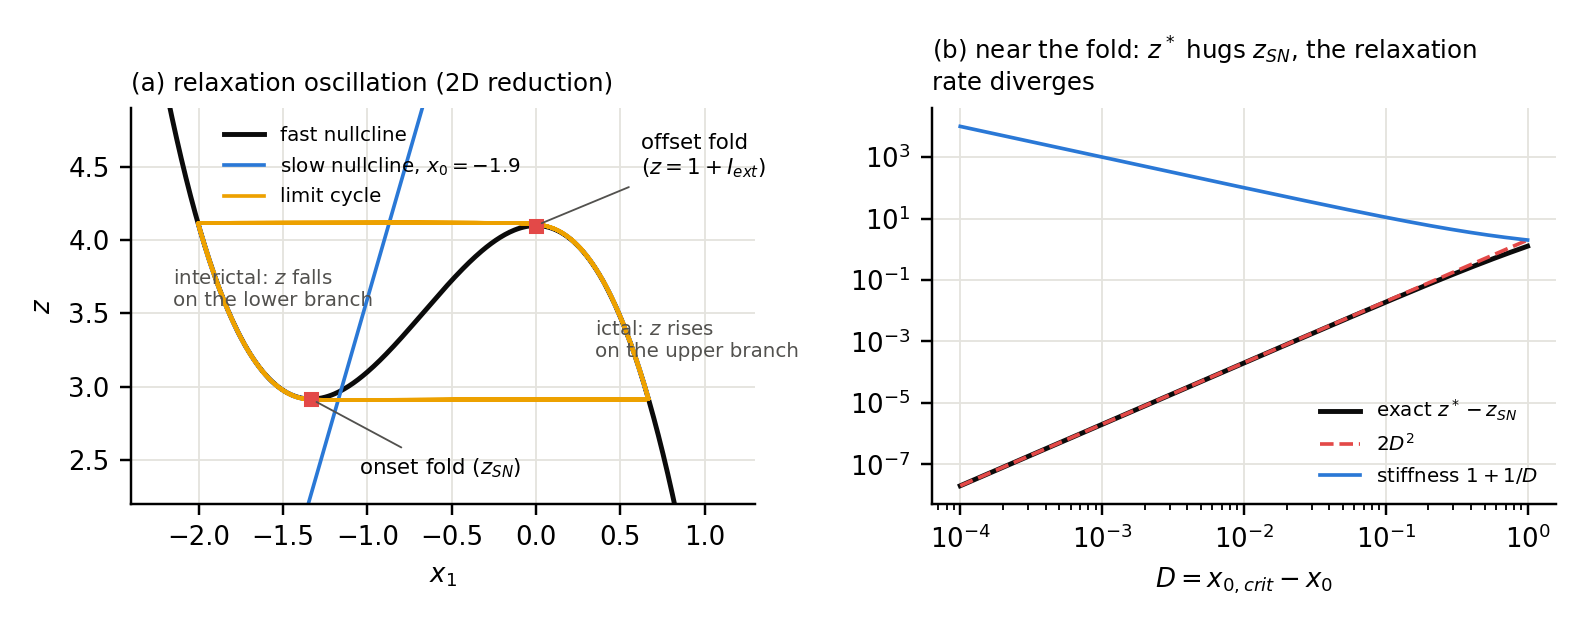
\includegraphics[width=\linewidth]{figs/th_relaxation.png}
\caption{(a) The 2D seizure cycle for $x_0=-1.9$. (b) Near the fold, the interictal fixed point lies only $2D^2$
above $\zsn$ (with $D = \xc - x_0$; Section~\ref{sec:nearfold}), and the effective relaxation rate of $z$ grows as
$1 + 1/D$: the dynamics become stiff precisely where the mapping is most interesting.}\label{fig:relax}
\end{figure}

\begin{figure}[H]\centering
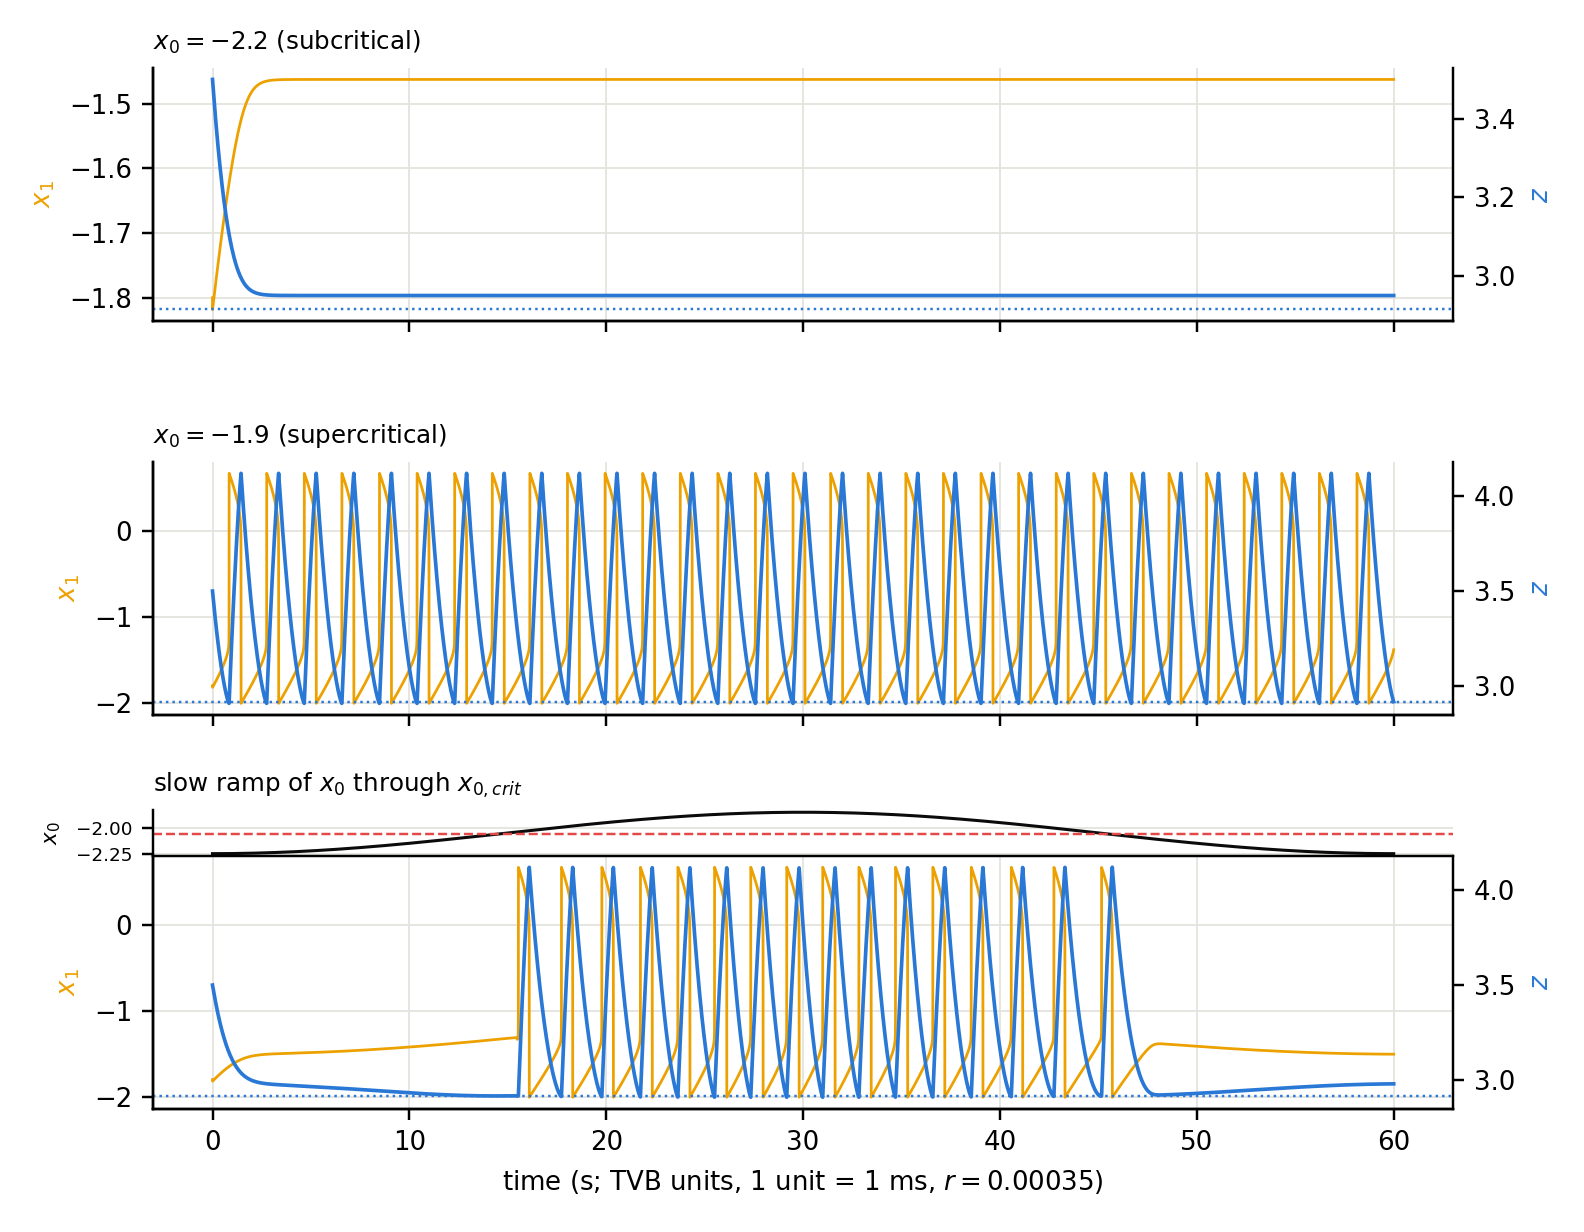
\includegraphics[width=0.95\linewidth]{figs/th_2d_sims.png}
\caption{2D Epileptor time series (TVB units). Top: subcritical, rest. Middle: supercritical, periodic seizures; $z$
oscillates between $\zsn$ (dotted) and 4.1. Bottom: $x_0$ ramped slowly through $\xc$ (inset): seizures start shortly
after the crossing and stop shortly after the return.}\label{fig:2d}
\end{figure}

\subsection{Behaviour near the fold}\label{sec:nearfold}
Near the fold, expand the fast nullcline: $G(x_1) \approx \zsn + 2u^2$ with $u = x_1 - \xsn$ (since $G''/2 = 2$).
With $D = \xc - x_0$ and \eqref{eq:xc}, the slow nullcline is $z = 4u + \zsn + 4D$. The interictal intersection solves
$2u^2 = 4u + 4D$, i.e.\ $u = 1 - \sqrt{1+2D} \approx -D$, so
\begin{equation}
z^* - \zsn \approx 2D^2,\qquad \frac{\partial x_1}{\partial z}\Big|_{\text{branch}} = \frac{1}{G'(x_1^*)} \approx -\frac{1}{4D}.
\end{equation}
With $x_1$ slaved to the branch, $\dot z = r[4(x_1(z) - x_0) - z]$ relaxes at rate $r(1 - 4\,\partial x_1/\partial z)
\approx r(1 + 1/D)$. Two consequences: (i) the interictal $z$ barely moves (by $2D^2$) while $x_0$ approaches the threshold,
so $z$ is a poor indicator of proximity to onset; (ii) numerically, explicit time steps overshoot across the fold when
$D$ is small, which we hit in practice (Section~\ref{sec:zint}).

\subsection{Time scales}\label{sec:timescales}
With TVB's $r$, $1/r\approx2.9$\,s. A 2D seizure (one passage up the ictal branch) lasts well under a second, and the
whole cycle a couple of seconds (Fig.~\ref{fig:2d}). In the full model, seizures last $\sim0.7$\,s in TVB units
(Fig.~\ref{fig:6d}). Fitted to patients, the time axis is stretched so that seizures last tens of seconds.
Our network's seizures last about a minute, and its HSP changes over thousands of seconds.

%==========================================================================================
\section{The HSP network seen as a slow--fast system}
%==========================================================================================
\subsection{Reminder of the model}
100 conductance-based LIF excitatory cells and 25 inhibitory cells; each E cell receives its own Poisson drive
(36\,Hz untreated, 40\,Hz reference). HSP acts on each E cell's recurrent AMPA and GABA conductances through
gains $\kA,\kG\in[0,1]$:
\[
\dot \kA = \frac{(1-\kA)\,G_\uparrow}{\tau^{A}_{ins}} - \frac{\kA\,G_\downarrow}{\tau^{A}_{int}},\qquad
\dot \kG = \frac{(1-\kG)\,G_\downarrow}{\tau^{G}_{ins}} - \frac{\kG\,G_\uparrow}{\tau^{G}_{int}},
\]
where $G_\uparrow$ is a sigmoid that is on when the cell's estimated rate $\hat r$ is below $\sim1$\,Hz and
$G_\downarrow$ one that is on above $\sim3$\,Hz ($\hat r$ is a 100\,s leaky spike count). The four time constants are
250\,s in the runs analysed here.

\subsection{Its cycle in slow--fast language}\label{sec:slowfast}
\begin{itemize}
\item \textbf{Fast subsystem}: the spiking network at fixed $(\kA, \kG)$. For moderate gains it has a low-rate state
($\sim1$\,Hz). Near $\kA\to1$, $\kG\to0$ it becomes \emph{bistable}: a saturated state (E $\sim$ hundreds of Hz) coexists
with the low-rate one, and input noise can kick the network from one to the other. We measured this directly: with
HSP frozen at the state 5\,min before an onset, half of the probe runs ignited (Section~\ref{sec:res-sens}).
\item \textbf{Slow subsystem}: $(\kA,\kG)$. Under the 36\,Hz drive the low-rate state sits below the target band, so HSP
inserts AMPA and removes GABA over thousands of seconds, carrying the fast subsystem towards its bistable region.
\item \textbf{Onset}: noise-triggered jump to the saturated state once the low-rate state has become fragile.
\item \textbf{Offset}: in the saturated state $\hat r$ saturates within seconds, $G_\downarrow$ switches on and HSP
internalises AMPA ($\kA$ collapses within $\sim0.27\tau$, i.e.\ about a minute for $\tau=250$\,s). The saturated state disappears and the
network falls back to low rates, now with very low $\kA$ and high $\kG$: a deep post-ictal state from which HSP
recovers over $\sim$1500\,s.
\end{itemize}
The structure is the same as the Epileptor's: a fast bistable subsystem moved through its transitions by slow
variables, with a negative feedback that ends the seizure. The difference is that the HSP gains do both jobs: they
build the excitability up between seizures (an $x_0$-like role) and they terminate the seizure (a $z$-like role).

\begin{table}[H]\centering\small
\begin{tabular}{p{3.6cm}p{5.4cm}p{5.6cm}}
\toprule
 & Epileptor (2D) & HSP network \\
\midrule
fast state & $x_1$ & population firing state (low-rate / saturated) \\
excitability & parameter $x_0$ (fixed per region) & set by $(\kA,\kG)$, slowly varying \\
onset & $z$ reaches the fold $\zsn$ (deterministic) & noise-triggered ignition near the bistable region \\
termination & $z$ rises to the end of the ictal branch & HSP internalises AMPA ($\kA\downarrow$), raises $\kG$ \\
inter-seizure interval & set by $r$ and $x_0$ & set by the HSP recovery from the post-ictal state \\
\bottomrule
\end{tabular}
\caption{Correspondence of the two models.}
\end{table}

%==========================================================================================
\section{The mapping, step by step}
%==========================================================================================
\begin{figure}[H]\centering
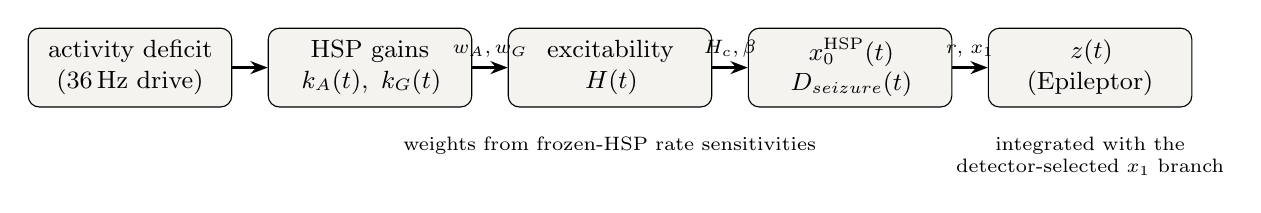
\begin{tikzpicture}[node distance=0.55cm and 0.45cm, every node/.style={font=\small},
  box/.style={draw, rounded corners, fill=boxc, align=center, minimum height=1.0cm, text width=2.35cm},
  arr/.style={-{Stealth[length=2.2mm]}, thick}]
\node[box] (d) {activity deficit\\(36\,Hz drive)};
\node[box, right=of d] (h) {HSP gains\\$\kA(t),\ \kG(t)$};
\node[box, right=of h] (H) {excitability\\$H(t)$};
\node[box, right=of H] (x0) {$\xh(t)$\\$D_{seizure}(t)$};
\node[box, right=of x0] (z) {$z(t)$\\(Epileptor)};
\draw[arr] (d) -- (h); \draw[arr] (h) -- node[above, font=\scriptsize]{$w_A, w_G$} (H);
\draw[arr] (H) -- node[above, font=\scriptsize]{$H_c, \beta$} (x0); \draw[arr] (x0) -- node[above, font=\scriptsize]{$r$, $x_1$} (z);
\node[below=0.25cm of H, font=\scriptsize, text width=6cm, align=center] {weights from frozen-HSP rate sensitivities};
\node[below=0.25cm of z, font=\scriptsize, text width=3.4cm, align=center] {integrated with the detector-selected $x_1$ branch};
\end{tikzpicture}
\caption{The chain of the mapping. Each arrow is a modelling step with its own assumptions.}
\end{figure}

\subsection{Why map HSP to $x_0$ rather than to $z$}
The 2D Epileptor has two slow quantities, and they do different jobs (Section~\ref{sec:fold}):
\begin{itemize}
\item $x_0$ is a \emph{parameter}. It sets where the slow nullcline $z=4(x_1-x_0)$ lies, and therefore whether the
fixed point sits on the interictal branch ($x_0<\xc$: the region rests) or not ($x_0>\xc$: the region seizes on its own).
\item $z$ is a \emph{state variable} with rate $r$. It runs each seizure: it falls slowly on the interictal branch, the
onset happens when it reaches $\zsn$, it rises on the ictal branch, and the offset happens when it reaches 4.1.
\end{itemize}
To decide which of the two the HSP state corresponds to, we compare three properties.

\textbf{(i) What HSP changes.} HSP multiplies the recurrent AMPA and GABA conductances onto E cells. It therefore changes
how strongly the network amplifies its own activity, and so whether a low-rate state can turn into runaway activity
without any change of input. This is the property that $x_0$ encodes (rest exists or not), not the one $z$ encodes
(where the system is inside a seizure cycle).

\textbf{(ii) How HSP moves in time.} Between two high-rate episodes, $\kA$ rises and $\kG$ falls over about an hour,
monotonically and with no fast component: this is the behaviour of a slowly varying parameter. $z$ cannot play that
role, because on these time scales it is not free. On the interictal branch it relaxes to its fixed point
$z^*(x_0)$ at rate $r(1+1/D)\ge r = 0.35$\,s$^{-1}$ (Section~\ref{sec:nearfold}), i.e.\ within seconds, while HSP takes
thousands of seconds. Between seizures, therefore, $z(t)\approx z^*(x_0(t))$: $z$ follows whatever $x_0$ does and carries
no information of its own. Mapping HSP to $z$ with a constant $x_0$ would mean forcing $z$ away from the value its own
equation imposes, and would leave $x_0$ with nothing in the data to set it.

\textbf{(iii) What remains testable.} If HSP sets $x_0(t)$, then $z(t)$ is not chosen but computed from the Epileptor
equation. Whether that computed $z$ behaves like the network (onsets at the right times) is a test of the mapping
rather than an assumption.

We therefore map the HSP state to a time-varying excitability $\xh(t)$ and reconstruct $z$.

\subsection{An excitability coordinate from local sensitivities}\label{sec:Hderiv}
We want one number $H(\kA,\kG)$ that summarises how far the HSP state pushes the network towards higher activity.
We ask four things of it:
\begin{enumerate}[label=(P\arabic*)]
\item $H$ increases with $\kA$ (more excitation) and decreases with $\kG$ (more inhibition);
\item the relative weight of AMPA and GABA comes from the spiking network, not from a choice;
\item $H=0$ at a reference state, so that $H$ measures a change;
\item $H$ stays usable far from that reference: over the untreated cycle $\kA$ goes from 0.16 to 0.98 and $\kG$
from 0.02 to 0.84.
\end{enumerate}
The construction below has eight steps. Steps 1--6 build $H$ from a local linearisation, step 7 discusses using it
globally, and step 8 checks it on numbers.

\paragraph{Step 1: the function that is linearised.}
Freeze HSP (all four time constants set to $10^{99}$\,s), set every E cell's gains to $(\kA,\kG)$, drive the network at
36\,Hz and measure its mean E rate over a window after a transient. Call the result
\[
\bar r_E(\kA,\kG) \quad [\mathrm{Hz}].
\]
Freezing is needed because with HSP on the gains move during the measurement, and the measured rate would not be a
function of one pair $(\kA,\kG)$. $\bar r_E$ is the input--output response of the fast subsystem (Section~\ref{sec:slowfast}) at fixed slow
variables. It is only defined where the low-rate state survives the whole window. If
the frozen network ignites (E rate $>10$\,Hz in a 1\,s bin), it never comes back, because HSP is frozen, and the run says
nothing about the local rate response. Such runs are excluded and counted.

\paragraph{Step 2: first-order expansion in the gains.}
Let $(\kA^{ref},\kG^{ref})$ be a reference state. Taylor's theorem in two variables gives
\begin{equation}
\bar r_E(\kA,\kG) = \bar r_E^{ref} + S_A\,(\kA-\kA^{ref}) + S_G\,(\kG-\kG^{ref}) + O\!\left(|\Delta k|^2\right),
\label{eq:lin}\end{equation}
\[
S_A = \frac{\partial\bar r_E}{\partial\kA}\Big|_{ref},\qquad S_G = \frac{\partial\bar r_E}{\partial\kG}\Big|_{ref}.
\]
We expect $S_A>0$ and $S_G<0$. The analysis checks these signs and refuses to compute weights when they fail.

\paragraph{Step 3: why $S_A$ and $S_G$ cannot be compared directly.}
$S_A$ and $S_G$ are in Hz per unit of gain. At the reference state used here, $\kA^{ref}=0.926$ and $\kG^{ref}=0.071$.
The same absolute step $\Delta k=0.01$ is a 1.1\% change of $\kA$ but a 14\% change of $\kG$. Comparing $S_A$ with $S_G$
would therefore compare a small relative change of excitation with a large relative change of inhibition. What is
comparable is the response to the same \emph{relative} change of each gain.

Relative changes are also the coordinates in which the HSP equations are simplest. Divide the HSP equations by $\kA$
and by $\kG$:
\begin{align*}
\frac{d\ln\kA}{dt} &= \frac{(1-\kA)\,G_\uparrow}{\kA\,\tau^{A}_{ins}} - \frac{G_\downarrow}{\tau^{A}_{int}},\\
\frac{d\ln\kG}{dt} &= \frac{(1-\kG)\,G_\downarrow}{\kG\,\tau^{G}_{ins}} - \frac{G_\uparrow}{\tau^{G}_{int}}.
\end{align*}
Look at a cell that is firing far above target ($G_\uparrow\approx0$, $G_\downarrow\approx1$). The first line becomes
$d\ln\kA/dt = -1/\tau^A_{int}$, a constant: AMPA internalisation lowers $\ln\kA$ at a fixed rate, whatever the current
$\kA$. Likewise, a silent cell ($G_\uparrow\approx1$, $G_\downarrow\approx0$) lowers $\ln\kG$ at the fixed rate
$1/\tau^G_{int}$. In $\ln k$, the removal halves of HSP are uniform drifts, and equal steps of $\ln k$ correspond to equal
durations of removal. The insertion halves are not uniform in $\ln k$ (they are uniform in $\ln(1-k)$). The log is
therefore an exact description of the removal phases and an approximation during build-up; step 7 checks whether this
matters.

\paragraph{Step 4: the same expansion in log-gains.}
Change variables to $u=\ln\kA$, $v=\ln\kG$, so $\kA=e^u$, $\kG=e^v$. By the chain rule,
\[
\frac{\partial\bar r_E}{\partial u} = \frac{\partial\bar r_E}{\partial\kA}\,\frac{d\kA}{du} = S_A\,\kA,\qquad
\frac{\partial\bar r_E}{\partial v} = S_G\,\kG .
\]
Evaluated at the reference, define the two \emph{log-sensitivities}, both positive:
\begin{equation}
q_A := \kA^{ref}\,S_A > 0,\qquad q_G := -\kG^{ref}\,S_G > 0 .
\end{equation}
The first-order expansion in $(u,v)$ is then
\begin{equation}
\bar r_E \approx \bar r_E^{ref} + q_A\,\ln\frac{\kA}{\kA^{ref}} - q_G\,\ln\frac{\kG}{\kG^{ref}} .
\label{eq:loglin}\end{equation}
$q_A$ is the rate change, in Hz, per unit change of $\ln\kA$; equivalently, $q_A/100$ is the change for a 1\% increase of
all AMPA gains. Equations \eqref{eq:lin} and \eqref{eq:loglin} agree to first order, because
$\ln(\kA/\kA^{ref}) = \Delta\kA/\kA^{ref} - \tfrac12(\Delta\kA/\kA^{ref})^2+\dots$. They differ at second order: they are
two different extrapolations of the same local slope. \eqref{eq:loglin} would be exact for a rate of the form
$a + q_A\ln\kA - q_G\ln\kG$.

\paragraph{Step 5: what is measured, and how precisely.}
The probe perturbs each gain by a fraction $\delta$ and takes a central difference:
\[
\bar r_E\big(\kA^{ref}(1\pm\delta),\kG^{ref}\big) = \bar r_E^{ref} \pm S_A\kA^{ref}\delta
+ \tfrac12\,\partial^2_{\kA}\bar r_E\,(\kA^{ref}\delta)^2 \pm O(\delta^3),
\]
so the second-order terms cancel in the difference and
\begin{equation}
q_A = \frac{\bar r_E(\kA^{ref}(1+\delta)) - \bar r_E(\kA^{ref}(1-\delta))}{2\delta} + O(\delta^2),\qquad
S_A = q_A/\kA^{ref},
\end{equation}
and likewise for GABA. Dividing by $2\delta$ is the same as dividing by $\ln(1+\delta)-\ln(1-\delta) = 2\delta+O(\delta^3)$,
so this is directly a derivative in $\ln k$. The $+$ and $-$ runs of a pair use the same Poisson input spike trains
(common random numbers). The input noise is then nearly identical in both runs and largely cancels in the difference:
for two runs with rate variance $\sigma^2$ and correlation $\rho$, the variance of the difference is $2\sigma^2(1-\rho)$
instead of $2\sigma^2$.

The choice of $\delta$ is a trade-off. A small $\delta$ keeps the $O(\delta^2)$ error small but makes the rate
difference $2\delta q$ small compared with the noise. A large $\delta$ moves the network far enough that it can
ignite. The numbers are (seed 1, 200\,s of measurement, 100 E cells, so one spike $= 5\times10^{-5}$\,Hz):
\begin{itemize}
\item AMPA: $S_A = 0.793$\,Hz at $\delta=2\%$, so $q_A = 0.926\times0.793 = 0.734$\,Hz and the measured difference is
$2\delta q_A = 0.029$\,Hz, about 590 spikes. This is well resolved ($S_A = 0.79$--$0.88$\,Hz for $\delta = 1$--$5\%$).
\item GABA: $S_G = -0.035$\,Hz at $\delta=2\%$, so $q_G = 0.071\times0.035 = 0.0025$\,Hz and $2\delta q_G = 1.0\times10^{-4}$\,Hz:
\textbf{two spikes} in the whole measurement. At $\delta=1\%$ the difference is also two spikes; at $5\%$ the sign of
$S_G$ is wrong (noise); at $10\%$, 2 of 10 runs ignited.
\end{itemize}
The GABA response is therefore at the resolution limit of the probe. What is robust is that it is very small, not its
exact value: at every state and seed probed, $w_G$ (defined in step 6) is between 0.002 and 0.017. The final weights
use $\delta=2\%$, the smallest perturbation at which both signs are as expected.

\paragraph{Step 6: normalisation.}
Divide \eqref{eq:loglin} by $q_A+q_G$ and define $H$ as the normalised predicted change:
\begin{equation}\boxed{\;H := \frac{\bar r_E^{lin}-\bar r_E^{ref}}{q_A+q_G}
= w_A\ln\frac{\kA}{\kA^{ref}} - w_G\ln\frac{\kG}{\kG^{ref}},\qquad
w_{A} = \frac{q_A}{q_A+q_G},\quad w_G = \frac{q_G}{q_A+q_G}\;}\label{eq:H}\end{equation}
With $q_A=0.734$\,Hz and $q_G=0.0025$\,Hz: $w_A = 0.9966$, $w_G = 0.0034$.

The division does not lose or add information downstream. Suppose $H$ is multiplied by any constant $c>0$. $H_c$ is
computed from $H$ (Section~\ref{sec:Hc}), so it is multiplied by $c$ too, and $H-H_c$ becomes $c(H-H_c)$. In the map
$\xh = \xc + \beta(H-H_c)$ (Section~\ref{sec:map}) this is the same as replacing $\beta$ by $c\beta$, and $\beta$ is not
calibrated anyway. The signs of all distances are unchanged. The only information the weights carry is therefore their
ratio, $w_G/w_A = q_G/q_A = 0.0034$. The normalisation simply fixes the scale so that $H$ is dimensionless,
$w_A+w_G=1$, and $H\approx\ln(\kA/\kA^{ref})$ when GABA is negligible. (P1)--(P3) hold by construction.

\paragraph{Step 7: using $H$ far from the reference (P4).}
\eqref{eq:H} is evaluated along the whole cycle, not only near the reference. Two facts help to see what this assumes.
First, \eqref{eq:H} can be rewritten as
\[
H = \ln\!\left[\Big(\frac{\kA}{\kA^{ref}}\Big)^{w_A}\Big(\frac{\kG}{\kG^{ref}}\Big)^{-w_G}\right]:
\]
$H$ is the log of a weighted ratio of excitatory to inhibitory gain. Second, in the plane $(\ln\kA,\ln\kG)$, $H$ is a
linear function: its level sets are parallel straight lines, and its gradient has the fixed direction $(w_A,-w_G)$.
Using $H$ globally therefore assumes that the \emph{direction} in which excitability increases is the same everywhere
on the cycle. It does not assume that the rate itself follows \eqref{eq:loglin} far away.

This assumption can be checked by repeating the probe at other states ($\delta=5\%$): post-ictal ($\kA=0.23$,
$\kG=0.77$) $w_A=0.983$; recovery ($0.80, 0.20$) $0.998$; early build-up ($0.93, 0.06$) $0.989$; the median interictal
state of seeds 2--5, $0.993$--$0.997$. The direction is stable: $w_A$ stays between 0.98 and 1.00. The
\emph{magnitude} is not. The post-ictal $q_A$ is $0.229\times0.255=0.058$\,Hz, against 0.734\,Hz at the reference, so
far from the reference $H$ is a coordinate that orders states, not a prediction of the rate. At the pre-ictal state,
5 of 10 probe runs ignited and no weight could be computed. This is a direct sign that the frozen network is bistable
there (Section~\ref{sec:res-sens}).

\paragraph{Step 8: worked examples (seed 1).}
\begin{center}\small
\begin{tabular}{lccccc}
\toprule
state & $\kA$ & $\kG$ & $w_A\ln(\kA/\kA^{ref})$ & $-w_G\ln(\kG/\kG^{ref})$ & $H$\\
\midrule
reference (median interictal) & 0.926 & 0.071 & 0 & 0 & 0\\
pre-ictal (onset $-$ 300\,s) & 0.972 & 0.025 & $+0.048$ & $+0.004$ & $+0.052$\\
40\,Hz network (median) & 0.752 & 0.215 & $-0.207$ & $-0.004$ & $-0.211$\\
post-ictal (end $+$ 300\,s) & 0.229 & 0.771 & $-1.394$ & $-0.008$ & $-1.402$\\
\bottomrule
\end{tabular}
\end{center}
The GABA term never exceeds 0.008, so $H$ is in practice $\ln(\kA/\kA^{ref})$. The pre-ictal value, 0.052, is the value
$H_c$ found in the next section (0.051).

\textbf{Assumptions built into $H$.}
(a) First order: a single slope per gain. (b) One reference state; the direction is checked at other states (step 7).
(c) The response is the \emph{mean rate} of the low-rate state, not the probability of ignition. This last assumption
fails for benzo (Section~\ref{sec:interp}): clamping $\kG=1$ barely changes the mean rate, but it prevents ignition.

\subsection{The critical value $H_c$}\label{sec:Hc}
$H$ says how excitable the HSP state is, but not where the threshold lies. The threshold is taken from the network's
own onsets.
\begin{enumerate}
\item \textbf{Onsets.} $t_j$ is the first 1\,s bin of seizure $j$ in which the E rate exceeds 10\,Hz (12 untreated
seizures after the 500\,s settling, 5 seeds).
\item \textbf{Pre-onset value.} $H_{c,j} = \mathrm{median}\{H(t):\ t\in[t_j-300\,\mathrm s,\ t_j-2\,\mathrm s),\ t \text{ not
ictal}\}$. The window is 300\,s because $H$ changes very little on the late plateau, so a long window averages out
fluctuations without mixing in the build-up; the last 2\,s are excluded because the gains already start to react to
the rising rate there. The median is used to be robust to a few outlying samples.
\item \textbf{Threshold.} $H_c = \mathrm{median}_j\,H_{c,j}$. The 12 values range from 0.024 to 0.058; $H_c = 0.0511$
(IQR 0.042--0.054). It changes by less than 0.002 for windows of 100\,s (0.0519) or 600\,s (0.0499).
\item \textbf{Leave-one-out.} To ask whether $H$ approaches the threshold before seizure $j$ without using seizure $j$
to set that threshold, we use $H_c^{(-j)} = \mathrm{median}_{i\neq j}H_{c,i}$ and $D_j(t) = H_c^{(-j)}-H(t)$.
\end{enumerate}
In gains: with GABA negligible, $H=H_c$ means $\kA \approx \kA^{ref}e^{H_c/w_A} = 0.926\,e^{0.0513} = 0.975$. This is
the observed plateau value of $\kA$ before onsets (0.97--0.98).

\subsection{From $H$ to the Epileptor: $\xh$, $D_{seizure}$, $D_H$}\label{sec:map}
We need a map $\varphi$ from $H$ to $x_0$. It should be increasing (more excitable network, larger $x_0$), and it should
send the network's threshold to the Epileptor's: $\varphi(H_c) = \xc$. Any smooth such map can be expanded around
$H_c$:
\[
\varphi(H) = \xc + \varphi'(H_c)\,(H-H_c) + O\big((H-H_c)^2\big).
\]
Keeping the first order gives the affine map, with $\beta := \varphi'(H_c) > 0$:
\begin{equation}
\xh(t) = \xc + \beta\,[H(t) - H_c],\qquad
D_{seizure}(t) = \xc - \xh(t) = \beta\,[H_c - H(t)],\qquad D_H(t) = H_c - H(t).
\end{equation}
\textbf{What would fix $\beta$.} A second state with both a known $H_2$ and a justified Epileptor value $x_{0,2}$ would
give $\beta = (x_{0,2}-\xc)/(H_2-H_c)$. The 40\,Hz network is the obvious candidate ($H=-0.211$), but nothing assigns
an Epileptor $x_0$ to ``healthy'': any value below $\xc$ would be consistent with it never seizing. We therefore set
$\beta=1$, meaning one unit of $H$ is drawn as one unit of $x_0$, \emph{only as a visual embedding}.

\textbf{What is and is not meaningful with $\beta=1$.}
\begin{itemize}
\item The \textbf{sign}: $\mathrm{sign}(D_{seizure}) = \mathrm{sign}(\beta)\,\mathrm{sign}(H_c-H) = \mathrm{sign}(D_H)$
for any $\beta>0$. Subcritical ($D>0$), critical ($D=0$) and supercritical ($D<0$) do not depend on $\beta$.
\item The \textbf{ordering} of states along $x_0$ does not depend on $\beta$ either: post-ictal ($x_0=-3.52$) $<$ 40\,Hz
network ($-2.32$) $<$ plateau ($\approx-2.06$).
\item The \textbf{size} of $D_{seizure}$ in Epileptor units does depend on $\beta$, and so does everything in the Epileptor
that depends on it. Near the fold the interictal $z^*$ sits $2D^2$ above $\zsn$ and relaxes at rate $r(1+1/D)$
(Section~\ref{sec:nearfold}), so the reconstructed $z$ values and the positions of the nullclines in the figures scale
with $\beta$.
\item $D_{seizure}$ is a distance to a bifurcation, \emph{not} a time to seizure.
\end{itemize}
Worked example: post-ictal, $\xh = -2.062 + (-1.402 - 0.051) = -3.515$; 40\,Hz, $-2.062 + (-0.211-0.051) = -2.324$, so
$D_{seizure} = +0.262$; pre-ictal, $-2.062 + 0.001 = -2.061$, essentially at the threshold.

\subsection{What plays the role of $x_1$}
The $z$ equation needs $x_1(t)$, but the network has no Epileptor variable. Building one from the firing rate would
need an arbitrary midpoint and amplitude. Instead, $x_1$ is the Epileptor's own coordinate, and the network's seizure
detector only chooses the branch. For a given $z$, the fast nullcline condition $G(x_1)=z$ is the cubic
\[
-x_1^3 - 2x_1^2 + 1 + I_{ext} - z = 0 .
\]
For $\zsn < z < 4.1$ it has three real roots: a lower one ($x_1<-4/3$, interictal branch, attracting), a middle one
($-4/3<x_1<0$, repelling) and an upper one ($x_1>0$, ictal branch, attracting). The roots are computed numerically, and
\[
x_1(t) = \begin{cases} \text{lower root at } z(t), & \text{detector: interictal},\\
\text{upper root at } z(t), & \text{detector: ictal.}\end{cases}
\]
The middle root is never used, because the fast dynamics leave it. No new parameter enters. If the requested branch
does not exist at the current $z$ (interictal while $z<\zsn$, ictal while $z>4.1$), $x_1$ is held at that branch's fold
and the sample is flagged. Such samples mark where the network's state and the Epileptor geometry disagree.

\subsection{Reconstructing $z(t)$}\label{sec:zint}
\[
\dot z = r\,h(z,t),\qquad h(z,t) = 4\big(x_1(z,t) - \xh(t)\big) - z - 0.1 z^7\mathbf 1_{z<0},\qquad r = 0.35\ \mathrm{s}^{-1}.
\]
TVB's $r=0.00035$\,ms$^{-1}$ is converted to the data's unit (seconds). $\xh$ is linearly interpolated between the 1\,s
samples, and $z(0)$ is the interictal fixed point for $\xh(0)$; the first 500\,s are discarded anyway.

\textbf{Why an explicit step fails here.} The first implementation used an explicit (exponential-Euler) step of 0.1\,s.
13\% of the untreated samples then fell below $\zsn$ while the network was interictal and $D_{seizure}>0$, which would
wrongly read as ``supercritical''. The cause is the slope of the lower branch. Differentiating $G(x_1(z)) = z$ gives
$dx_1/dz = 1/G'(x_1)$, and $G'\to0$ at the fold, so $dx_1/dz$ diverges as $z\to\zsn$. An explicit step uses the slope
at the start of the step. Near the fold that slope changes by a large factor within one step, so the step overshoots
to $z<\zsn$, where the lower branch no longer exists, and the next step comes back: $z$ chatters across the fold. The
linear rate makes the same point: the interictal relaxation rate is $r(1+1/D)$ (Section~\ref{sec:nearfold}). For
$D=0.017$ this is $0.35\times60 = 21$\,s$^{-1}$, so a 0.1\,s step spans two relaxation times.

\textbf{Why backward Euler with bisection works.} The backward-Euler update is
\[
z_{n+1} = z_n + \Delta t\,r\,h(z_{n+1}, t_{n+1}) \iff F(z_{n+1}) = 0,\qquad F(z) := z - z_n - \Delta t\,r\,h(z,t_{n+1}).
\]
$h$ is strictly decreasing in $z$, term by term:
\begin{itemize}
\item on either attracting branch, $dx_1/dz = 1/G'(x_1)$ with $G'(x_1) = -3x_1^2-4x_1 = -x_1(3x_1+4)$. For $x_1<-4/3$,
$-x_1>0$ and $3x_1+4<0$, so $G'<0$; for $x_1>0$, $-x_1<0$ and $3x_1+4>0$, so $G'<0$. Hence $4\,dx_1/dz<0$;
\item at a clamp, $x_1$ is constant, so this term contributes 0;
\item $-z$ has derivative $-1$;
\item $-0.1z^7\mathbf 1_{z<0}$ has derivative $-0.7z^6\le0$ for $z<0$ and 0 otherwise, and is continuous at 0.
\end{itemize}
So $\partial_z h \le -1 < 0$ and $F'(z) = 1 - \Delta t\,r\,\partial_z h \ge 1 + \Delta t\,r > 0$: $F$ is strictly increasing
and has exactly one root, which bisection finds to machine precision once a bracket is found ($F\to\pm\infty$ as
$z\to\pm\infty$). For a linearised $h = -\lambda(z-z^*)$, the backward-Euler factor is $1/(1+\Delta t\,r\lambda)$, which is
in $(0,1)$ for every step size: the scheme cannot overshoot, however stiff the fold. With $\Delta t=0.1$\,s, the
interictal $z$ agrees with $\Delta t=0.02$\,s to $10^{-5}$. The largest difference, $5\times10^{-2}$, occurs at the 1\,s
jumps between branches.

%==========================================================================================
\section{Results}
%==========================================================================================
Data: the long runs behind the paper results (HSP $\tau=250$\,s, 15\,000\,s, 5 seeds), for the untreated (cyclic)
network, the 40\,Hz reference (stable), DBS 60\,pA and benzo. 12 untreated seizures (2, 2, 3, 2, 3 per seed); no
seizure in the other conditions.

\begin{figure}[H]\centering
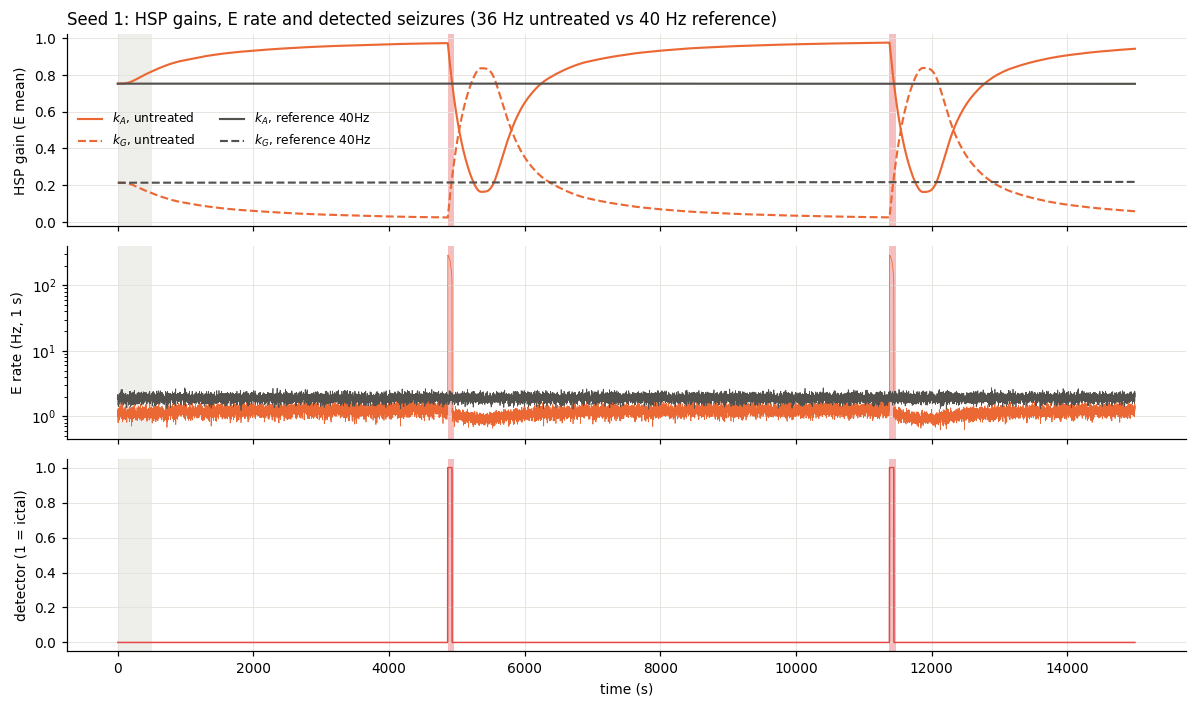
\includegraphics[width=0.95\linewidth]{figs/nb_cell07_0.png}
\caption{Seed 1. HSP gains (solid $\kA$, dashed $\kG$), E rate and detector, untreated (orange) vs reference (grey).
Between seizures $\kA$ climbs towards 1 and $\kG$ falls towards 0; each seizure inverts them.}
\end{figure}

\subsection{Sensitivities and weights}\label{sec:res-sens}
\begin{table}[H]\centering\footnotesize
\setlength{\tabcolsep}{3.5pt}
\begin{tabular}{lcccccccc}
\toprule
state & seed & $\delta$ & $\kA$ & $\kG$ & $\bar r_E$ (Hz) & $S_A$ (Hz) & $S_G$ (Hz) & $w_A$ \\
\midrule
median interictal & 1 & 1\% & 0.926 & 0.071 & 1.25 & $0.878\pm0.024$ & $-0.071$ & 0.994 \\
median interictal & 1 & 2\% & 0.926 & 0.071 & 1.25 & $0.793\pm0.016$ & $-0.035$ & \textbf{0.997} \\
median interictal & 1 & 5\% & 0.926 & 0.071 & 1.25 & $0.826\pm0.015$ & $+0.018\pm0.053$ & -- (sign) \\
median interictal & 1 & 10\% & 0.926 & 0.071 & 1.25 & ignites (2/10 runs) & $-0.016\pm0.027$ & -- \\
post-ictal (+300\,s) & 1 & 5\% & 0.229 & 0.771 & 0.94 & $0.255\pm0.001$ & $-0.0013$ & 0.983 \\
recovery (+1500\,s) & 1 & 5\% & 0.798 & 0.201 & 1.16 & $0.584\pm0.007$ & $-0.004$ & 0.998 \\
early build-up & 1 & 5\% & 0.928 & 0.063 & 1.25 & $0.846\pm0.012$ & $-0.136\pm0.056$ & 0.989 \\
pre-ictal ($-300$\,s) & 1 & 5\% & 0.972 & 0.025 & 1.29 & ignites (5/10 runs) & -- & -- \\
median, seeds 2--5 & 2--5 & 5\% & 0.89--0.93 & 0.07--0.11 & 1.22--1.25 & 0.73--0.80 & $-0.02$ to $-0.07$ & 0.993--0.997 \\
\bottomrule
\end{tabular}
\caption{Frozen-HSP rate sensitivities. Error bars from two noise seeds (none shown when both seeds gave the same
spike counts). The final weights use $\delta=2\%$, where both signs are as expected; at 5\% the GABA derivative is
within noise of zero.}\label{tab:sens}
\end{table}

\begin{figure}[H]\centering
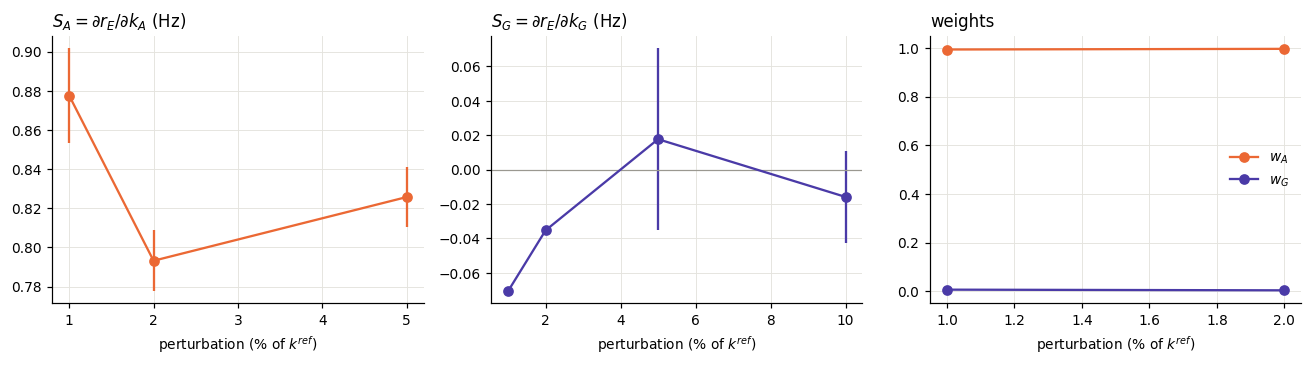
\includegraphics[width=0.95\linewidth]{figs/nb_cell12_0.png}
\caption{$S_A$, $S_G$ and the weights against perturbation size (seed 1, median interictal state). Points with
an ignited run are missing.}
\end{figure}

\textbf{Reading.} $S_A\approx0.8$\,Hz per unit of $\kA$ is stable across 1--5\% and across seeds. $S_G$ is tiny: at the
interictal state, $\kG\approx0.07$, so the GABA conductance onto E cells is $\sim0.07$\,nS, and changing it by 2\% shifts the
mean rate by one or two spikes in 200\,s. The weights are therefore $w_A = 0.997$, $w_G = 0.003$: $H\approx\ln(\kA/\kA^{ref})$.
Even at the post-ictal state ($\kG = 0.77$), $w_G$ is only 0.02. Finally, two probes \emph{ignited}: the frozen network at
the state 5\,min before an onset, and $\kA$ raised by 10\% from the median state. Near $H_c$ the frozen spiking network is
itself bistable, so a local derivative of the mean rate is not even defined there.

\subsection{$H_c$, $\xh$ and the distances over time}
$H_{c,j}$ over the 12 seizures: median $H_c = 0.0511$ (IQR 0.042--0.054); 0.0519, 0.0511, 0.0499 for pre-onset windows
of 100, 300 and 600\,s. With $\xc=-2.06204$, $\zsn = 2.91481$.

\begin{figure}[H]\centering
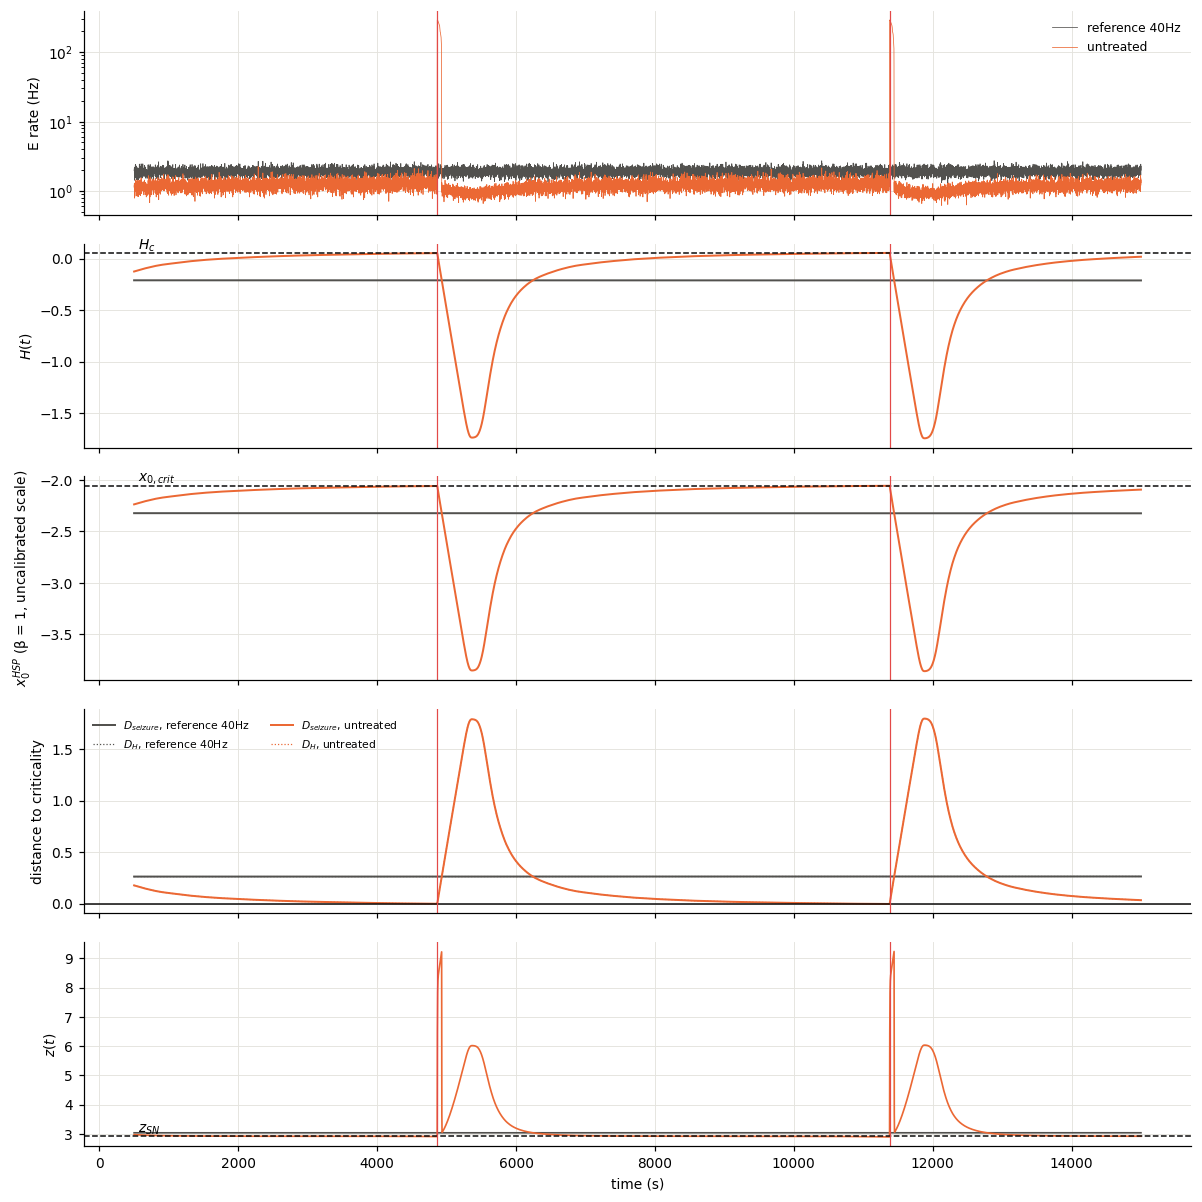
\includegraphics[width=0.92\linewidth]{figs/nb_cell23_0.png}
\caption{Seed 1, untreated (orange) vs reference (grey). From top: E rate; $H(t)$ with $H_c$ (dashed); $\xh(t)$ with
$\xc$; $D_{seizure}$ (solid) and $D_H$ (dotted; identical for $\beta=1$); reconstructed $z$ with $\zsn$. Red lines:
seizure onsets.}\label{fig:ts}
\end{figure}

\subsection{The trajectory in $(\xh, z)$}
\begin{figure}[H]\centering
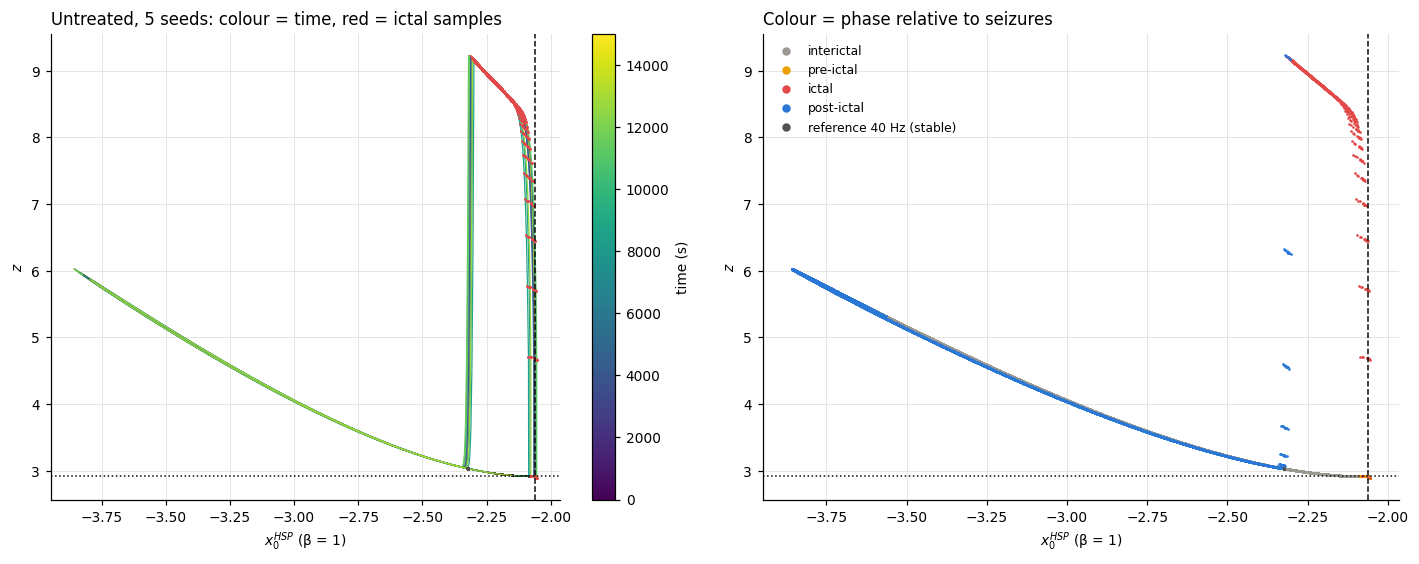
\includegraphics[width=\linewidth]{figs/nb_cell25_0.png}
\caption{Main result: the untreated trajectory of all 5 seeds in $(\xh, z)$, coloured by time (left) and by phase
(right), with the 40\,Hz reference (dark grey cluster, left of $\xc$). Dashed: $\xc$; dotted: $\zsn$.}\label{fig:traj}
\end{figure}

\textbf{How to read Fig.~\ref{fig:traj}.} The loop runs clockwise:
\begin{enumerate}
\item \emph{Build-up} (grey): along the lower curve, $\xh$ rises slowly from $\sim-3.9$ to $\xc$ over $\sim$1 hour, and $z$
follows its quasi-static value $z^*(\xh)$ down to $\zsn$.
\item \emph{Onset} (orange then red) at $\xh\approx\xc$: the detector switches $x_1$ to the ictal branch, and $z$ shoots up to
$\sim9$.
\item \emph{Ictal leg} (red): during the $\sim1$\,min seizure, HSP collapses $\kA$, so $\xh$ moves left to $\sim-2.3$
while $z$ stays high.
\item \emph{Post-ictal} (blue): the seizure ends, $z$ drops back onto the curve, and $\xh$ keeps falling, to $\sim-3.9$, as
$\kA$ reaches its minimum; then the build-up starts again.
\end{enumerate}

\begin{figure}[H]\centering
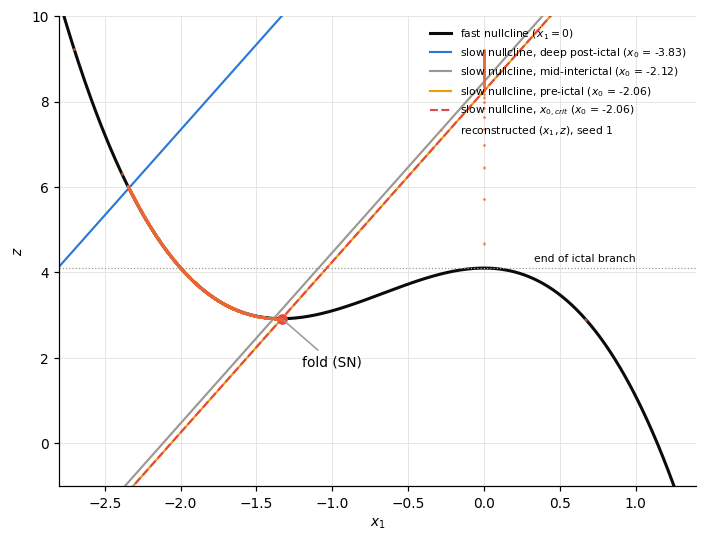
\includegraphics[width=0.62\linewidth]{figs/nb_cell27_0.png}
\caption{Canonical phase plane with slow nullclines for representative $\xh$ values from the untreated trajectory
(deep post-ictal, mid-interictal, pre-ictal $\approx\xc$) and the reconstructed $(x_1,z)$ of seed 1 (orange dots).
HSP sweeps the slow nullcline far to the left after a seizure and slowly back to the fold.}
\end{figure}

\subsection{Stable vs cyclic, with the same mapping}
\begin{figure}[H]\centering
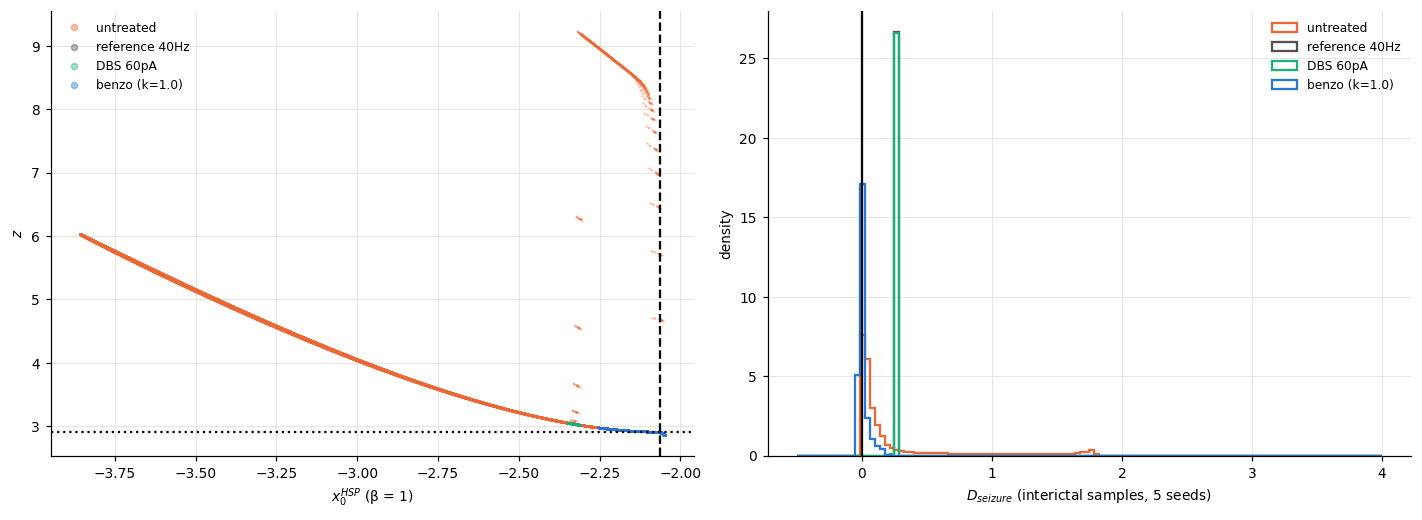
\includegraphics[width=\linewidth]{figs/nb_cell29_0.png}
\caption{All conditions with the identical mapping. Left: $(\xh, z)$. Right: distribution of $D_{seizure}$ on
interictal samples (5 seeds).}
\end{figure}
\begin{table}[H]\centering\small
\begin{tabular}{lcccc}
\toprule
condition & median $D_{seizure}$ & minimum & share $D<0$ & seizures \\
\midrule
untreated & $+0.059$ & $-0.007$ & 4.4\% & 12 \\
reference 40\,Hz & $+0.262$ & $+0.258$ & 0 & 0 \\
DBS 60\,pA & $+0.257$ & $+0.250$ & 0 & 0 \\
benzo ($\kG=1$) & $-0.007$ & $-0.014$ & 63.8\% & 0 \\
\bottomrule
\end{tabular}
\caption{Distance to criticality on interictal samples ($\beta=1$; signs meaningful).}\label{tab:D}
\end{table}

\subsection{Quantitative answers}
\begin{figure}[H]\centering
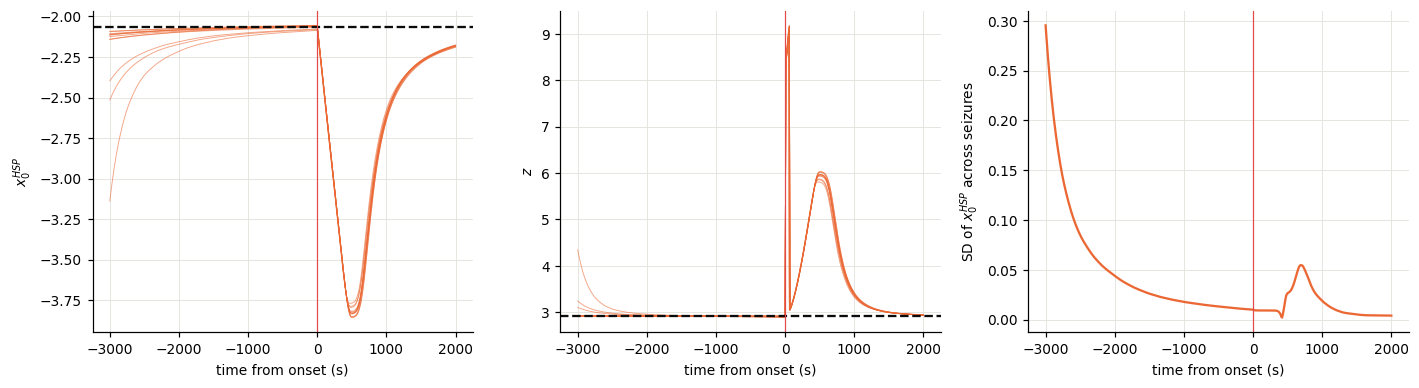
\includegraphics[width=\linewidth]{figs/nb_cell32_0.png}
\caption{Onset-aligned $\xh$ (left) and $z$ (middle) for all 12 seizures, and the across-seizure SD of $\xh$ (right).}
\end{figure}

\begin{enumerate}
\item \textbf{A repeatable loop.} Across seizures, $\xh$ differs by 0.018 (SD) at $-1000$\,s, 0.010 at $-100$\,s and 0.026 at
$+500$\,s, against a cycle range of 1.8 ($-3.86$ to $-2.05$). Every cycle follows the same path.
\item \textbf{The stable condition stays subcritical.} The reference and DBS 60\,pA sit in a narrow band at
$D_{seizure}\approx+0.26$ and never approach the fold.
\item \textbf{$\xh$ reaches $\xc$ at onset.} With a leave-one-out $H_c$, the median $D_{seizure}$ at onset is $-0.001$. In 6 of
12 seizures, $D\le0$ was reached 9--19\,min before onset; the other 6 started while $D$ was still slightly positive
($0.002$--$0.025$).
\item \textbf{Closer before seizures.} In all 12 seizures, $D$ in the last 5\,min (median $\approx0.000$) is smaller than in a
matched window 25--30\,min earlier (median $+0.018$); Wilcoxon $p=0.0005$.
\item \textbf{The post-ictal leg moves away.} $D$ increases by a median of 1.35 over the first 10\,min after each seizure.
\item \textbf{Robustness.} $w_A$ is 0.98--1.00 across perturbation sizes, cycle states and seeds; $H_c$ changes by less than
0.002 for pre-onset windows of 100--600\,s; $z(0)$ is forgotten within 4--8\,s. The flagged samples (interictal $x_1$ held
at the fold because $z<\zsn$) make up 5.8\% of untreated time, roughly consistent with the 4.4\% of interictal time at $D<0$
plus the ictal samples beyond the end of the ictal branch.
\end{enumerate}

%==========================================================================================
\section{Interpretation}\label{sec:interp}
%==========================================================================================
\subsection{What the loop means}
The HSP state, expressed as an Epileptor excitability, carries the network back and forth through the Epileptor's
seizure threshold. After each seizure it throws the network deep into the subcritical region (far from the fold), and
over about an hour it brings it back exactly to $\xc$, where the seizure occurs. The trajectory is the same in every
cycle and every seed. In Epileptor terms, our untreated network is not a region with a fixed epileptogenic $x_0$:
it is a region whose $x_0$ is itself a slow variable, regulated by homeostasis, that \emph{returns to criticality}. The
healthy reference has a fixed $x_0$ well below the threshold.

\subsection{HSP plays both roles}
In the Epileptor, the build-up and the termination are done by different objects: $x_0$ sets whether seizures can
happen, and $z$ times each seizure. In the network, HSP does both:
\begin{itemize}
\item between seizures it is the slow drift of $x_0$ towards the threshold;
\item during a seizure it is the negative feedback that ends it: the ictal leg of the loop is $\xh$ moving to the
subcritical side within a minute.
\end{itemize}
The reconstructed $z$ confirms that the Epileptor's own clock does not fit: during seizures it climbs to $\sim9$, far
past the end of the ictal branch (4.1) where the Epileptor would already have ended the seizure within seconds. With
TVB's $r$, $z$ is three orders of magnitude faster than HSP, so between seizures it is simply slaved to $\xh$
($|z - z^*(\xh)|$ below 0.02 for 99\% of interictal samples; 0.16 with $r$ ten times smaller; it lags by up to $\sim1$
after seizures only with $r$ a hundred times smaller). And near the fold, $z^*$ moves only by $2D^2$, so $z$ carries
almost no information about proximity to onset. In this model, the $(\xh, z)$ plane is effectively one-dimensional
between seizures.

\subsection{Deterministic threshold vs noisy onset}
The 2D Epileptor seizes as soon as $x_0>\xc$. The network spent up to 19\,min at $D_{seizure}<0$ before seizing (4.4\%
of untreated interictal time), and half of its seizures started slightly before $D$ reached zero. Both point to
noise-triggered transitions near a fold: in the frozen probes, the pre-ictal state ignites in half of the runs.
Near $\xc$, the network has a seizure \emph{rate}, not a seizure time. This is the same conclusion as the LFP analysis:
no early-warning trend in the last 10 minutes, but a long high-risk state that a slow observable can track.

\subsection{Where the mapping fails: inhibition and benzo}
GABA receives almost no weight, because at interictal states $\kG$ is so low that its local effect on the mean E rate is
negligible. As a consequence, benzo ($\kG$ clamped at 1, with $\kA$ saturating at 0.999) is mapped \emph{beyond} the
threshold for 64\% of the time, yet it never seized in $5\times20\,000$\,s. The mean-rate sensitivity misses what
inhibition does to \emph{ignition}: strong inhibition keeps the saturated state from being reached even when excitation
is maximal. The excitability that matters for seizures is not the slope of the mean rate but the stability of the
low-rate state. A sensitivity based on ignition (for example, the probability that a frozen state ignites within a
fixed time, or the size of perturbation needed to ignite it) would very likely give GABA a real weight and classify benzo
as subcritical.

\subsection{What is anchored and what is not}
\begin{itemize}
\item \textbf{Anchored in the spiking model}: the relative weight of AMPA and GABA (local rate sensitivities), the critical
value $H_c$ (HSP state before detected onsets, consistent with the frozen-network ignition), seizure times.
\item \textbf{Anchored in the Epileptor}: $\xc$, $\zsn$ and the fold geometry, computed from its equations with TVB defaults.
\item \textbf{Phenomenological}: $\beta=1$ (the size of the $x_0$ axis), TVB's $r$ (which makes $z$ fast), and $x_1$ (the
canonical branch chosen by the detector, not a measured network variable).
\end{itemize}

%==========================================================================================
\section{Limitations and next steps}
%==========================================================================================
\textbf{Limitations.}
\begin{itemize}
\item One reference state for the weights. The weights barely change along the cycle for the mean rate, but this is
because the mean rate is the wrong quantity near ignition.
\item $\beta$ is uncalibrated, so distances in Epileptor units are not comparable with $x_0$ values inferred in patients.
\item $x_1$ is not measured; it is chosen by the detector. The mapping therefore cannot predict seizure times, only
place the observed ones.
\item The 2D reduction has no fast ictal oscillation and a fold instead of a homoclinic offset; comparing waveforms
(e.g.\ the LFP proxy against $x_2 - x_1$) would need the full model.
\item Post hoc only: nothing is fed back into the network.
\end{itemize}

\textbf{Next steps}, in order of expected value:
\begin{enumerate}
\item \textbf{Ignition-based weights.} Replace $\bar r_E$ by an ignition measure (probability of ignition within a fixed
time with HSP frozen, over many noise seeds) and recompute $w_A$, $w_G$. Test: does benzo become subcritical?
\item \textbf{A second anchor for $\beta$.} For example, map the frozen-network ignition probability as a function of $H$
onto the Epileptor's response to noise as a function of $x_0$, which would fix the scale.
\item \textbf{A slower $z$, or a different $z$.} Fit $r$ to the network's seizure duration; or identify $z$ with a separate
fast component of HSP (the rate estimator or the collapse of $\kA$ during the seizure) instead of TVB's clock.
\item \textbf{Closed loop.} Drive an Epileptor with $\xh(t)$ plus noise and compare its seizure times with the network's;
or feed the Epileptor's $z$ back into the network as an extra slow variable.
\item \textbf{Inference from observables.} Estimate $\xh$ from the LFP power below 30\,Hz (which tracks $\kA$), in the spirit of
the Virtual Epileptic Patient's inference of $x_0$ from recordings.
\end{enumerate}

\appendix
\section{Implementation details}
\begin{itemize}
\item Notebook: \path{epilepsy/HSP_Epileptor_trajectory.ipynb} (runs top to bottom from a clean kernel; all analysis
parameters in one configuration cell). Probe runner: \path{epilepsy/hsp_epileptor_probe.py}; probe results cached in
\path{results_hsp_epileptor/probes.json} (114 runs).
\item Data: \texttt{seed\_robustnessv2/results/lfp\_tau250\_15k/raw/}: E-mean $\kA,\kG$ and E rate every 1\,s.
\item Fast-nullcline roots: closed-form cubic (trigonometric form for three real roots, Cardano otherwise).
\item $z$: backward Euler, $\Delta t=0.1$\,s, exact bisection; $\xh$ linearly interpolated.
\item Theory figures: \texttt{HSP\_Epileptor\_report/theory\_figures.py} (LSODA; TVB parameter values).
\end{itemize}

\begin{thebibliography}{99}\small
\bibitem{jirsa2014} V.~K. Jirsa, W.~C. Stacey, P.~P. Quilichini, A.~I. Ivanov, C.~Bernard. On the nature of seizure
dynamics. \emph{Brain} 137:2210--2230, 2014.
\bibitem{proix2014} T.~Proix, F.~Bartolomei, P.~Chauvel, C.~Bernard, V.~K. Jirsa. Permittivity coupling across brain
regions determines seizure recruitment in partial epilepsy. \emph{Journal of Neuroscience} 34:15009--15021, 2014.
\bibitem{jirsa2017} V.~K. Jirsa, T.~Proix, D.~Perdikis, et al. The Virtual Epileptic Patient: individualized whole-brain
models of epilepsy spread. \emph{NeuroImage} 145:377--388, 2017.
\bibitem{proix2017} T.~Proix, F.~Bartolomei, M.~Guye, V.~K. Jirsa. Individual brain structure and modelling predict
seizure propagation. \emph{Brain} 140:641--654, 2017.
\bibitem{saggio2020} M.~L. Saggio, D.~Crisp, J.~M. Scott, et al. A taxonomy of seizure dynamotypes. \emph{eLife}
9:e55632, 2020.
\bibitem{izhikevich2000} E.~M. Izhikevich. Neural excitability, spiking and bursting. \emph{International Journal of
Bifurcation and Chaos} 10:1171--1266, 2000.
\bibitem{sanzleon2013} P.~Sanz Leon, S.~A. Knock, M.~M. Woodman, et al. The Virtual Brain: a simulator of primate brain
network dynamics. \emph{Frontiers in Neuroinformatics} 7:10, 2013.
\bibitem{krupa2001} M.~Krupa, P.~Szmolyan. Relaxation oscillation and canard explosion. \emph{Journal of Differential
Equations} 174:312--368, 2001.
\bibitem{kuehn2015} C.~Kuehn. \emph{Multiple Time Scale Dynamics}. Springer, 2015.
\end{thebibliography}
\end{document}
